% GNUPLOT: LaTeX picture with Postscript
\begingroup
  \makeatletter
  \providecommand\color[2][]{%
    \GenericError{(gnuplot) \space\space\space\@spaces}{%
      Package color not loaded in conjunction with
      terminal option `colourtext'%
    }{See the gnuplot documentation for explanation.%
    }{Either use 'blacktext' in gnuplot or load the package
      color.sty in LaTeX.}%
    \renewcommand\color[2][]{}%
  }%
  \providecommand\includegraphics[2][]{%
    \GenericError{(gnuplot) \space\space\space\@spaces}{%
      Package graphicx or graphics not loaded%
    }{See the gnuplot documentation for explanation.%
    }{The gnuplot epslatex terminal needs graphicx.sty or graphics.sty.}%
    \renewcommand\includegraphics[2][]{}%
  }%
  \providecommand\rotatebox[2]{#2}%
  \@ifundefined{ifGPcolor}{%
    \newif\ifGPcolor
    \GPcolortrue
  }{}%
  \@ifundefined{ifGPblacktext}{%
    \newif\ifGPblacktext
    \GPblacktextfalse
  }{}%
  % define a \g@addto@macro without @ in the name:
  \let\gplgaddtomacro\g@addto@macro
  % define empty templates for all commands taking text:
  \gdef\gplbacktext{}%
  \gdef\gplfronttext{}%
  \makeatother
  \ifGPblacktext
    % no textcolor at all
    \def\colorrgb#1{}%
    \def\colorgray#1{}%
  \else
    % gray or color?
    \ifGPcolor
      \def\colorrgb#1{\color[rgb]{#1}}%
      \def\colorgray#1{\color[gray]{#1}}%
      \expandafter\def\csname LTw\endcsname{\color{white}}%
      \expandafter\def\csname LTb\endcsname{\color{black}}%
      \expandafter\def\csname LTa\endcsname{\color{black}}%
      \expandafter\def\csname LT0\endcsname{\color[rgb]{1,0,0}}%
      \expandafter\def\csname LT1\endcsname{\color[rgb]{0,1,0}}%
      \expandafter\def\csname LT2\endcsname{\color[rgb]{0,0,1}}%
      \expandafter\def\csname LT3\endcsname{\color[rgb]{1,0,1}}%
      \expandafter\def\csname LT4\endcsname{\color[rgb]{0,1,1}}%
      \expandafter\def\csname LT5\endcsname{\color[rgb]{1,1,0}}%
      \expandafter\def\csname LT6\endcsname{\color[rgb]{0,0,0}}%
      \expandafter\def\csname LT7\endcsname{\color[rgb]{1,0.3,0}}%
      \expandafter\def\csname LT8\endcsname{\color[rgb]{0.5,0.5,0.5}}%
    \else
      % gray
      \def\colorrgb#1{\color{black}}%
      \def\colorgray#1{\color[gray]{#1}}%
      \expandafter\def\csname LTw\endcsname{\color{white}}%
      \expandafter\def\csname LTb\endcsname{\color{black}}%
      \expandafter\def\csname LTa\endcsname{\color{black}}%
      \expandafter\def\csname LT0\endcsname{\color{black}}%
      \expandafter\def\csname LT1\endcsname{\color{black}}%
      \expandafter\def\csname LT2\endcsname{\color{black}}%
      \expandafter\def\csname LT3\endcsname{\color{black}}%
      \expandafter\def\csname LT4\endcsname{\color{black}}%
      \expandafter\def\csname LT5\endcsname{\color{black}}%
      \expandafter\def\csname LT6\endcsname{\color{black}}%
      \expandafter\def\csname LT7\endcsname{\color{black}}%
      \expandafter\def\csname LT8\endcsname{\color{black}}%
    \fi
  \fi
  \setlength{\unitlength}{0.0500bp}%
  \begin{picture}(7200.00,5040.00)%
    \gplgaddtomacro\gplbacktext{%
      \csname LTb\endcsname%
      \put(145,887){\makebox(0,0)[r]{\strut{}-2}}%
      \put(671,790){\makebox(0,0)[r]{\strut{}-1.5}}%
      \put(1197,693){\makebox(0,0)[r]{\strut{}-1}}%
      \put(1724,597){\makebox(0,0)[r]{\strut{}-0.5}}%
      \put(2250,500){\makebox(0,0)[r]{\strut{} 0}}%
      \put(2776,404){\makebox(0,0)[r]{\strut{} 0.5}}%
      \put(3303,307){\makebox(0,0)[r]{\strut{} 1}}%
      \put(3828,211){\makebox(0,0)[r]{\strut{} 1.5}}%
      \put(4354,114){\makebox(0,0)[r]{\strut{} 2}}%
      \put(4638,193){\makebox(0,0)[l]{\strut{}-2}}%
      \put(4942,360){\makebox(0,0)[l]{\strut{}-1.5}}%
      \put(5246,527){\makebox(0,0)[l]{\strut{}-1}}%
      \put(5550,694){\makebox(0,0)[l]{\strut{}-0.5}}%
      \put(5853,861){\makebox(0,0)[l]{\strut{} 0}}%
      \put(6157,1029){\makebox(0,0)[l]{\strut{} 0.5}}%
      \put(6461,1196){\makebox(0,0)[l]{\strut{} 1}}%
      \put(6765,1363){\makebox(0,0)[l]{\strut{} 1.5}}%
      \put(7069,1530){\makebox(0,0)[l]{\strut{} 2}}%
      \put(154,1991){\makebox(0,0)[r]{\strut{}-0.5}}%
      \put(154,2187){\makebox(0,0)[r]{\strut{} 0}}%
      \put(154,2384){\makebox(0,0)[r]{\strut{} 0.5}}%
      \put(154,2580){\makebox(0,0)[r]{\strut{} 1}}%
      \put(154,2775){\makebox(0,0)[r]{\strut{} 1.5}}%
      \put(154,2971){\makebox(0,0)[r]{\strut{} 2}}%
      \put(154,3167){\makebox(0,0)[r]{\strut{} 2.5}}%
      \put(154,3363){\makebox(0,0)[r]{\strut{} 3}}%
      \put(154,3560){\makebox(0,0)[r]{\strut{} 3.5}}%
      \put(154,3756){\makebox(0,0)[r]{\strut{} 4}}%
      \put(154,3952){\makebox(0,0)[r]{\strut{} 4.5}}%
      \put(-641,3164){\makebox(0,0){\strut{}f(x,y)}}%
    }%
    \gplgaddtomacro\gplfronttext{%
      \put(6065,4316){\makebox(0,0)[r]{\strut{}$f(x,y)=\frac{1}{4} x^4 - \frac{1}{2}x^2 + \frac{1}{10}x + \frac{1}{2}y^2$}}%
      \csname LTb\endcsname%
      \put(6065,4096){\makebox(0,0)[r]{\strut{}       4}}%
      \csname LTb\endcsname%
      \put(6065,3876){\makebox(0,0)[r]{\strut{}       3}}%
      \csname LTb\endcsname%
      \put(6065,3656){\makebox(0,0)[r]{\strut{}       2}}%
      \csname LTb\endcsname%
      \put(6065,3436){\makebox(0,0)[r]{\strut{}       1}}%
      \csname LTb\endcsname%
      \put(6065,3216){\makebox(0,0)[r]{\strut{}       0}}%
      \csname LTb\endcsname%
      \put(1777,290){\makebox(0,0){\strut{}x}}%
      \put(6757,714){\makebox(0,0){\strut{}y}}%
      \put(-641,3164){\makebox(0,0){\strut{}f(x,y)}}%
    }%
    \gplbacktext
    \put(0,0){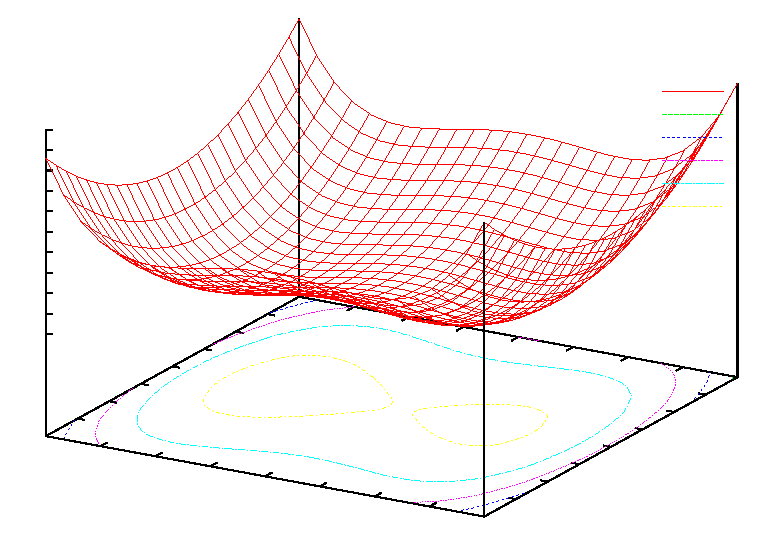
\includegraphics{graphics/aluffi02}}%
    \gplfronttext
  \end{picture}%
\endgroup
